\begin{frame}
    \frametitle{\problemtitle}
    \begin{block}{Problem}
        % TODO: Remove this comment when you're done writing the solutions.
        Given a tree and a set of extra edges (bridges), find the shortest tour
        through the extra edges, that uses each tree-edge at most once.
    \end{block}
\end{frame}

\begin{frame}
    \frametitle{\problemtitle}
    \begin{block}{Solution}
        \begin{itemize}
            \item<+-> Each tree edge connects two parts of the graph.
            \item<+-> If an odd number of bridges connect the two parts, the tree edge must be used in the optimal tour.
            \item<+-> The inverse is also true, if the number is even, the tree edge is not used in the shortest solution.
            \item<+-> Starting with leaves, count amount of bridges connected to that sub tree. Only the parity of this number matters.
            \item<+-> This gives an $\mathcal O(n)$ DFS solution.
        \end{itemize}
    \end{block}
    \centering
            \hfill
            \onslide<1->{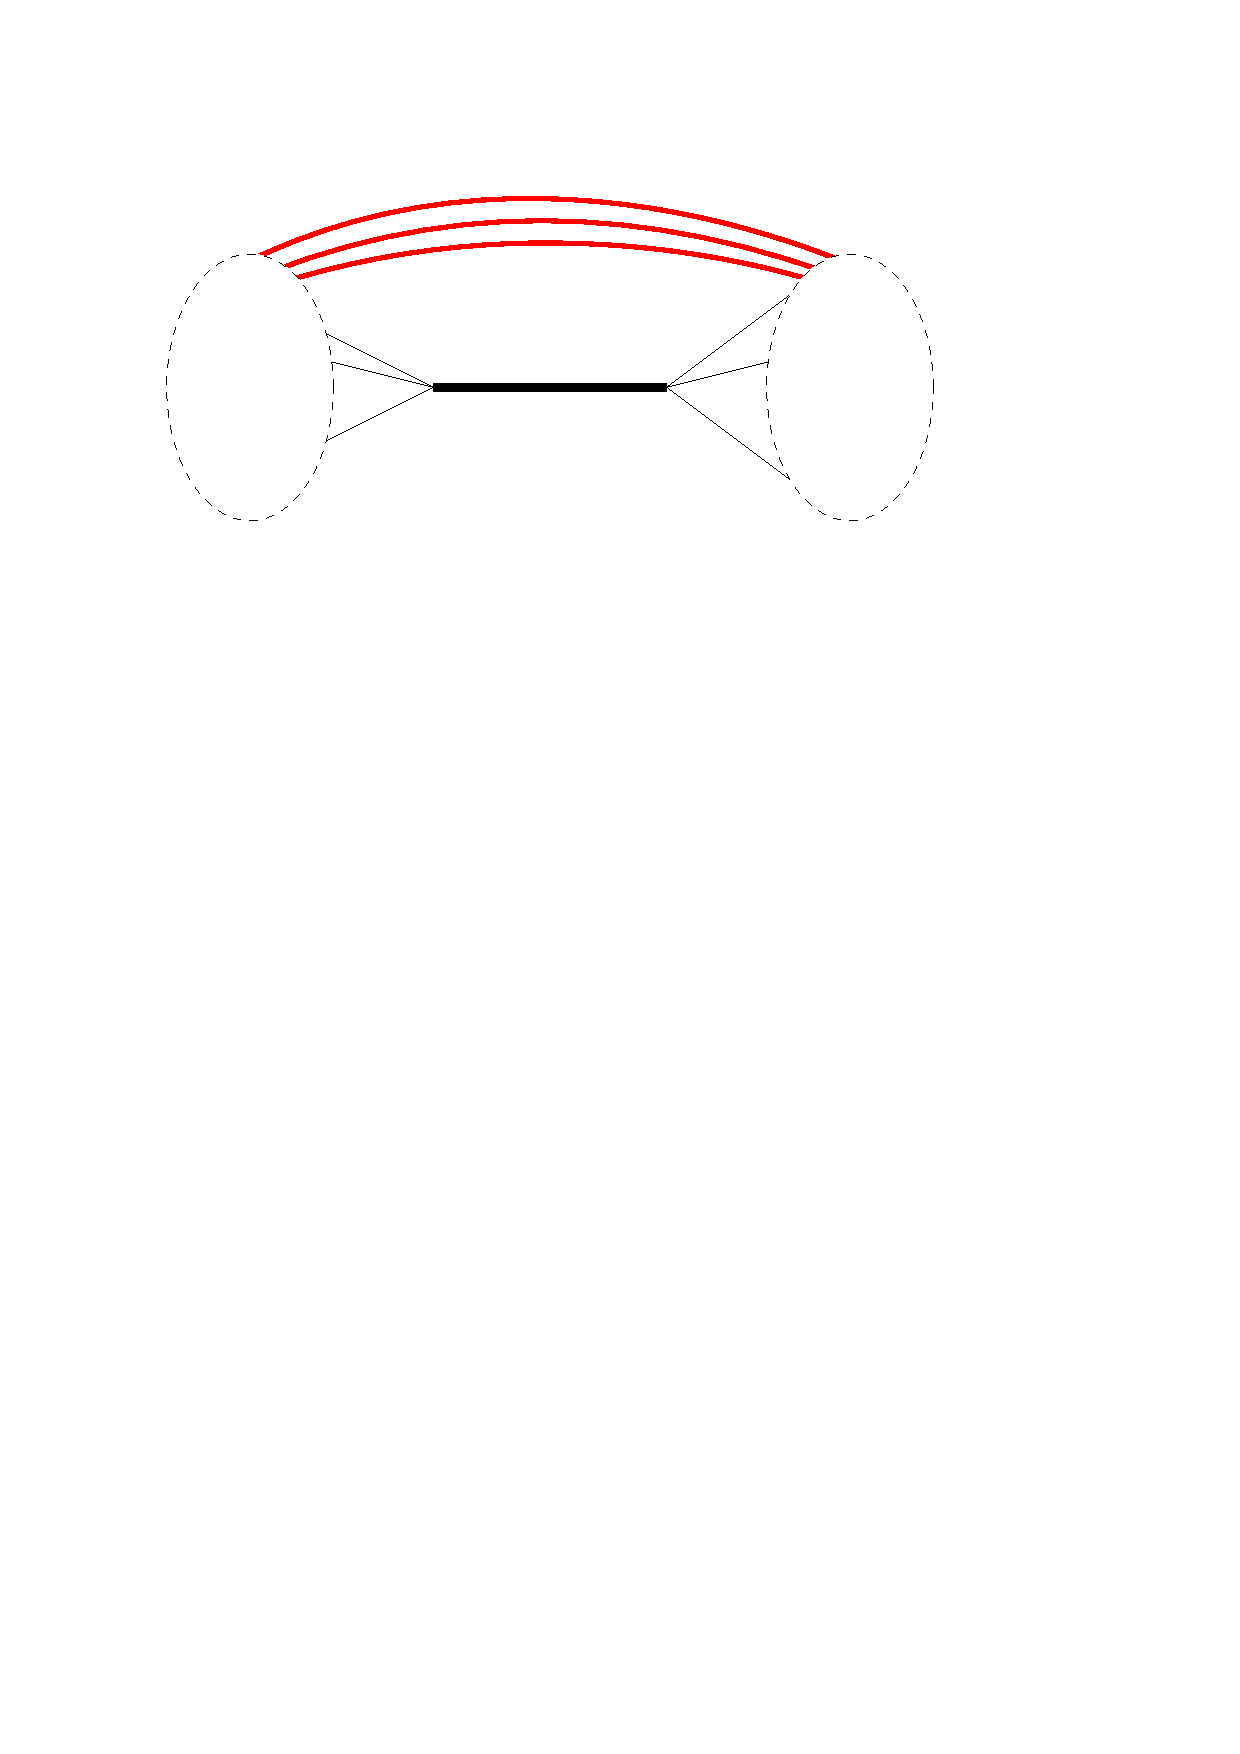
\includegraphics[width=5cm]{odd-bridges.pdf}}
            \hfill
            \onslide<3->{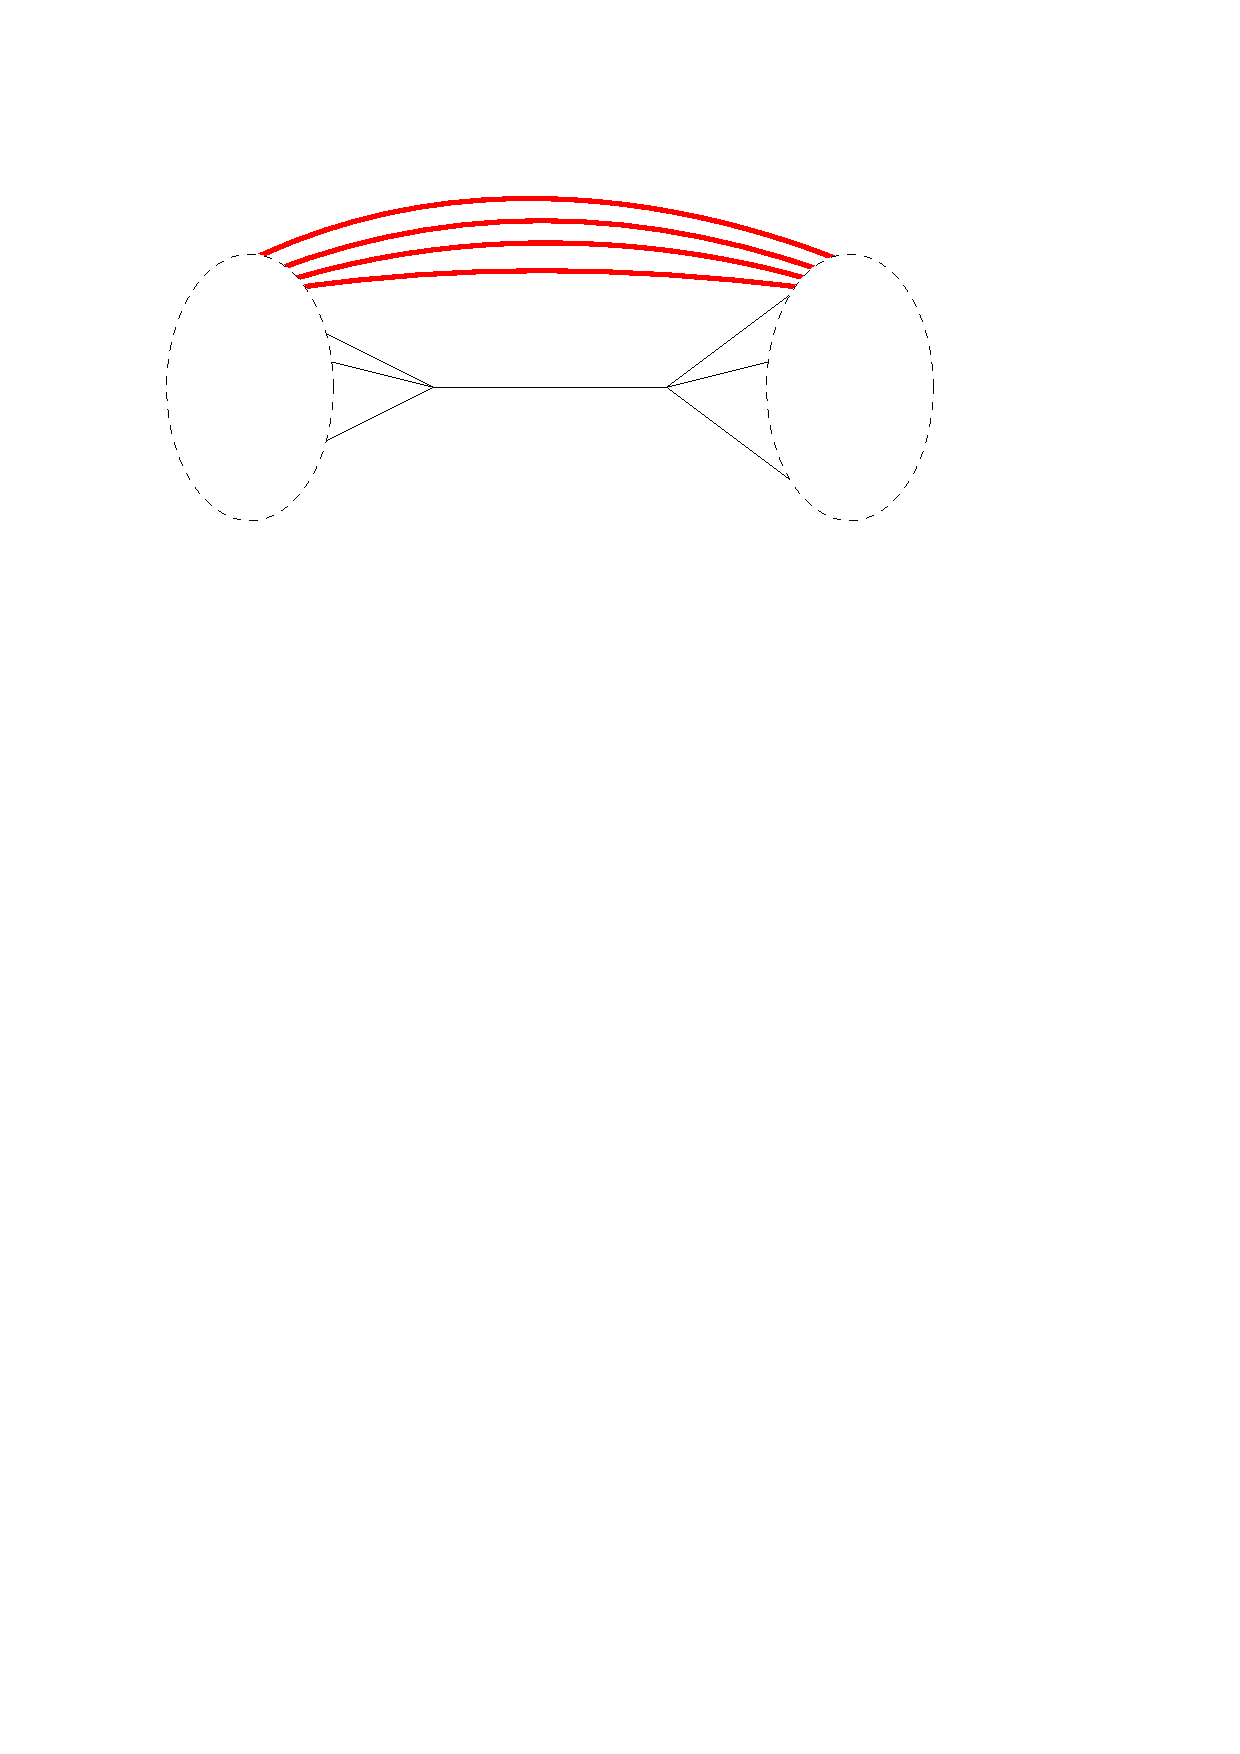
\includegraphics[width=5cm]{even-bridges.pdf}}
            \hfill
            \hfill% Silly LaTeX, requiring \hfill twice at the end of a line
    \solvestats
\end{frame}
